\documentclass[a4paper,12pt]{article}
\usepackage[top=2.5cm,bottom=2.5cm,left=2.5cm,right=2.5cm]{geometry}
%% \usepackage[brazil,brazilian]{babel}
\usepackage{amsmath, nccmath}
\usepackage{amsfonts}
\usepackage{amssymb}
\usepackage{bm}
\usepackage{multirow}
\usepackage{natbib}
\usepackage[colorlinks,citecolor=blue,urlcolor=blue]{hyperref}
\usepackage[utf8]{inputenc}
\usepackage{graphicx}  
\usepackage{float}
\usepackage{pdflscape} % horizontal page
\usepackage{tabularx}
\usepackage[english,vlined,ruled]{algorithm2e}
\usepackage{booktabs}
\usepackage{tikz}
\usetikzlibrary{positioning,shapes,arrows}
\usepackage{adjustbox}
\usepackage{tikz}
\usetikzlibrary{backgrounds}
\usetikzlibrary{arrows}
\usetikzlibrary{shapes,shapes.geometric,shapes.misc}

% this style is applied by default to any tikzpicture included via \tikzfig
\tikzstyle{tikzfig}=[baseline=-0.25em,scale=0.5]

% these are dummy properties used by TikZiT, but ignored by LaTex
\pgfkeys{/tikz/tikzit fill/.initial=0}
\pgfkeys{/tikz/tikzit draw/.initial=0}
\pgfkeys{/tikz/tikzit shape/.initial=0}
\pgfkeys{/tikz/tikzit category/.initial=0}

% standard layers used in .tikz files
\pgfdeclarelayer{edgelayer}
\pgfdeclarelayer{nodelayer}
\pgfsetlayers{background,edgelayer,nodelayer,main}

% style for blank nodes
\tikzstyle{none}=[inner sep=0mm]

% include a .tikz file
\newcommand{\tikzfig}[1]{%
{\tikzstyle{every picture}=[tikzfig]
\IfFileExists{#1.tikz}
  {\input{#1.tikz}}
  {%
    \IfFileExists{./figures/#1.tikz}
      {\input{./figures/#1.tikz}}
      {\tikz[baseline=-0.5em]{\node[draw=red,font=\color{red},fill=red!10!white] {\textit{#1}};}}%
  }}%
}

% the same as \tikzfig, but in a {center} environment
\newcommand{\ctikzfig}[1]{%
\begin{center}\rm
  \tikzfig{#1}
\end{center}}

% fix strange self-loops, which are PGF/TikZ default
\tikzstyle{every loop}=[]

\usepackage{setspace}
\onehalfspacing

\title{
  
  A multinomial generalized linear mixed model for clustered competing
  risks data

}

\usepackage{authblk}

\author[1]{Henrique Aparecido Laureano
  \footnote{E-mail: henriqueaparecidolaureano@gmail.com}
}
\author[2]{Ricardo Rasmussen Petterle}
\author[3]{Guilherme Parreira da Silva}
\author[4]{Wagner Hubo Bonat}

\affil[1]{
  Instituto de Pesquisa Pel\'{e} Pequeno Pr\'{i}ncipe,
  Curitiba, Brasil
}
\affil[2]{
  Departamento de Medicina Integrada,
  Universidade Federal do Paran\'{a}, Curitiba, Brasil
}
\affil[3,4]{
  Laborat\'{o}rio de Estat\'{i}stica e Geoinforma\c{c}\~{a}o,
  Departamento de Estat\'{i}stica,
  Universidade Federal do Paran\'{a}, Curitiba, Brasil
}

\begin{document}
\maketitle

\begin{abstract}

  Clustered competing risks data are a complex failure time data
  scheme. Its main characteristics are the cluster structure, which
  implies a latent within-cluster dependence between its elements, and
  its multiple variables competing to be the one responsible for the
  occurrence of an event, the failure. To handle this kind of data, we
  propose a full likelihood approach, based on a generalized linear
  mixed model instead a usual complex frailty model. We model the
  competing causes in the probability scale, in terms of the cumulative
  incidence function (CIF). A multinomial distribution is assumed for
  the competing causes and censorship, conditioned on the latent
  effects. The latent effects are accommodated via a multivariate
  Gaussian distribution. The CIF is specified as the product of an
  instantaneous risk level function with a failure time trajectory level
  function. The estimation procedure is performed through the R package
  TMB (Template Model Builder), an \texttt{C++} based framework with
  efficient Laplace approximation and automatic differentiation
  routines. A large simulation study is performed, based on different
  latent structure formulations. The model presents to be of difficult
  estimation, with our results converging to a latent structure where
  both risk and failure time trajectory levels are correlated.

\end{abstract}
\vfill
\noindent\textbf{Keywords}: 
Clustered competing risks data;
Within-cluster dependence;
Multinomial generalized linear mixed model (GLMM);
TMB: Template Model Builder;
Laplace approximation;
Automatic differentiation (AD).
\vspace{0.2cm}
\newpage

\section{Introduction}

Competing risks data, and more generally failure time data, can be
modeled in two possible scales: the hazard and the probability scale,
with the former being the most popular. A competing risks process can be
seen as the multivariate extension of a failure time process, having
multiple causes competing to be the one responsible for the desired
event occurrence, properly, a failure. In \autoref{fig:crp} a visual aid
is provided considering \(m\) competing causes.

\begin{figure}[H]
 \centering
 \scalebox{0.85}{
  \begin{tikzpicture}
   \begin{pgfonlayer}{nodelayer}
    \node [style=circle,draw=black,fill=white] (7) at (-7.5, 5.5) {1};
    \node [style=circle,draw=black,fill=white] (9) at (-7.5, 4.5) {2};
    \node [style=none] (11) at (-7.5, 3.5) {$\vdots$};
    \node [style=circle,draw=black,fill=white] (12) at (-7.5, 2.5) {$m$};
    \node [style=circle,draw=black,fill=white] (14) at (-12.25, 4) {0};
    \node [style=none] (29) at (-11.75, 4.25) {};
    \node [style=none] (30) at (-8, 5.5) {};
    \node [style=none] (31) at (-8, 4.5) {};
    \node [style=none] (32) at (-8, 2.5) {};
    \node [style=none] (36) at (-11.75, 4) {};
    \node [style=none] (37) at (-11.75, 3.75) {};
   \end{pgfonlayer}
   \begin{pgfonlayer}{edgelayer}
	\draw [style=1side] (37.center) to (32.center);
	\draw [style=1side] (36.center) to (31.center);
	\draw [style=1side] (29.center) to (30.center);
   \end{pgfonlayer}
  \end{tikzpicture}
 }
 \caption{Illustration of competing risks process.}
 \label{fig:crp}
\end{figure}

Failure time data is the branch of Statistics responsible to handle
random variables describing the time until the occurrence of an event, a
failure \citep{kalb&prentice,hougaard00}. The time until a failure is
called survival experience, and is the modeling object. To accommodate
the number of possible causes for a failure there is the competing risks
data scheme. More specifically, its clustered version with groups of
elements sharing some non-observed latent dependence structure.

When this framework is applied in real-world situations, we have to be
able to handle with the nonoccurrence of the desired event, by any of
the competing causes, for, let us say, \textit{logistic reasons}
(short-time study and outside scope causes are some examples). This,
generally noninformative, nonoccurrence of the event is called
censorship.

When the elements under study are organized in clusters (a family,
e.g.), it opens space to what is called \textit{family studies}. In
family studies, the goal is to accommodate the non-observed latent
dependence and try to understand the relationship between the family
elements. In other words, how the occurrence of an event in a subject
affects the survival experience for the same or similar event in its
familiars.

The survival experiences is usually modeled in the hazard (failure rate)
scale, and with the latent within-cluster dependence accommodation we
have what is called a frailty model
\citep{frailty78,frailty79,liang95,petersen98}. The use of frailty
models implies in complicated likelihood functions and inference
routines done via elaborated and slow EM algorithms
\citep{nielsen92,klein92} or inefficient MCMC schemes
\citep{hougaard00}. With multiple survival experiences, the general idea
is the same but with even more elaborated likelihoods
\citep{prentice78,therneau00} or mixture model approaches
\citep{larson85,kuk92}.

When in the hazard scale, the interpretations are in terms of hazard
rates. A less usual scale but with a more appealing interpretation is
the probability scale. For competing risks data, the work on the
probability scale is done by means of the cumulative incidence function
(CIF) \citep{andersen12}, with the main modeling approach being the
subdistribution \citep{fine&gray}.

For clustered competing risks data there are some available options but
with a lack of predominance. The options vary in terms of likelihood
specification, with its majority being designed for bivariate CIFs,
where increasing the CIF's dimension is a limitation. Some of the
existing options are (i) nonparametric approaches
\citep{cheng07,cheng09}; (ii) linear transformation models
\citep{fine99,gerds12}; (iii) semiparametric approaches based on
composite likelihoods \citep{shih,SCHEIKE}, estimating equations
\citep{crossoddsratioSCHEIKE,cheng&fine}, copulas
\citep{semiparametricSCHEIKE}, and mixtures \citep{naskar05,shi13}.

Besides the interpretation, by modeling the CIF it is possible to
specify complex within-cluster dependence structures. We follow
\cite{SCHEIKE} and work with a CIF specification based on its
decomposition in instantaneous risk and failure time trajectory
functions, with both being cluster-specifics and possible correlated. As
a modeling framework, we use a generalized linear mixed model (GLMM)
specification. Through a GLMM we have a straightforward full likelihood
specification, easy to virtually extend to any number of competing
causes, and capable to allow for complex CIF structures. To make the
estimation and inferential process the most efficient as possible we
take advantage of state-of-art computational libraries and efficiently
implemented routines under the \texttt{TMB} \citep{TMB} package of the R
\citep{R21} statistical software.

The class of generalized linear models (GLMs) \citep{GLM72} is probably
the most popular statistical modelling framework. Despite its
flexibility, the GLMs are not suitable for dependent data. For the
analysis of such data, \cite{laird82} proposed the random effects
regression models for longitudinal/repeated-measures data, and
\cite{breslow93} presented the GLMMs for the analysis of non-Gaussian
outcomes. In this framework, we can accommodate all competing causes of
failure and censorship under a multinomial probability distribution. The
latent within-cluster dependence is accommodated via a multivariate
normal distribution, and the cause-specific CIFs via the model's link
function.

The main goal of this work is to propose a GLMM approach to handle
clustered competing risks data with a flexible within-cluster dependence
structure. The model specification and the inferential routine are much
simpler than the usually used approaches, increasing its practical
relevance. The latent effects, the key complicator factor, are handled
out by means of an efficient Laplace approximation and automatic
differentiation routines. The main contributions of this article are:
(i) introducing the modeling of cause/cluster-specific CIFs of clustered
competing risks data into an efficient implementation of the GLMMs
framework; (ii) performing a extensive simulation study to check the
properties of the maximum likelihood estimator to learn the
cause-specific CIF forms and the feasibility of the within-cluster
dependence structure.; (iii) providing R code and \texttt{C++}
implementation for the used GLMMs.

The work is organized as follows. Section \ref{model} presents the CIF
specification and the multinomial GLMM. Section \ref{inference} presents
the estimation and inferential routines. Section \ref{simulation}
presents the performed simulation studies to check the model
viability. Finally, the main contributions of the article are discussed
in Section \ref{discussion}.

\section{Model}
\label{model}

\subsection{Cluster-specific cumulative incidence function (CIF)}
\label{CIF}

Consider that the observed follow-up time of a subject is given by \(T =
\min(T^{\ast},C)\), where \(T^{\ast}\) denote the failure time and \(C\)
denote the censoring time. Given the possible covariates \(\bm{x}\), for
a cause-specific of failure \(k\), the cumulative incidence function
(CIF) is defined as
\begin{align*}
 F_{k}(t \mid \bm{x})
 = \mathbb{P}[T \leq t,~K = k \mid \bm{x}]
 &= \int_{0}^{t} f_{k}(z \mid \bm{x})~\text{d}z\\
 &= \int_{0}^{t} \lambda_{k}(z \mid \bm{x})~S(z \mid \bm{x})
  ~\text{d}z, \quad t > 0, \quad k = 1,~\dots,~K,
\end{align*}
where \(f_{k}(t \mid \bm{x})\) is the (sub)density for the time to a
type \(k\) failure. The subdensity is composed by the cause-specific
hazard function or process \(\lambda_{k}(t \mid \bm{x})\), representing
the instantaneous rate for failures of type \(k\) at time \(t\) given
\(\bm{x}\) and all other failure types (competing causes). If we sum up
all cause-specific hazard functions we get the overall hazard function
\(\lambda(t \mid \bm{x})\). From the overall hazard function we arrive
in the overall survival function,
\[
 S(t \mid \bm{x}) = \mathbb{P}[T > t \mid \bm{x}] =
 \exp\left\{-\int_{0}^{t} \lambda(z \mid \bm{x})~\text{d}z\right\},
\]
the second function that compose the subdensity \(f_{k}(t \mid
\bm{x})\). A comprehensive reference for all these definitions is
the book of \cite{kalb&prentice}.

To take into consideration our clustered/family structure, we follow the
same CIF specification of \cite{SCHEIKE}. For two competing causes of
failure, the cause-specific CIFs are specified in the following manner
\begin{equation}
 F_{k} (t \mid \bm{x},~u_{1},~u_{2},~\eta_{k}) =
 \underbrace{\pi_{k}(\bm{x},~u_{1},~u_{2})}_{
 \substack{\text{cluster-specific}\\\text{risk level}}}\times
  \underbrace{\Phi[w_{k} g(t) - \bm{x}\bm{\gamma}_{k} - \eta_{k}]}_{
   \substack{\text{cluster-specific}\\\text{failure time trajectory}}
  }, \quad t > 0, \quad k = 1,~2,
  \label{eq:cif}
\end{equation}
i.e., as the product of a cluster-specific risk level with a
cluster-specific failure time trajectory, resulting in a
cluster-specific CIF. What makes these components cluster-specific are
\(\bm{u} = \{u_{1},~u_{2}\}\) and \(\bm{\eta} =
\{\eta_{1},~\eta_{2}\}\), Gaussian distributed latent effects with zero
mean and potentially correlated,
\[
 \begin{bmatrix} u_{1}\\u_{2}\\\eta_{1}\\\eta_{2} \end{bmatrix} \sim
 \parbox{2.5cm}{\centering Multivariate Normal}
 \left(
  \begin{bmatrix} 0\\0\\0\\0\end{bmatrix},
  \begin{bmatrix}
   \sigma_{u_{1}}^{2}&
   \text{cov}(u_{1},~u_{2})&
   \text{cov}(u_{1},~\eta_{1})&\text{cov}(u_{1},~\eta_{2})\\
   &\sigma_{u_{2}}^{2}&
   \text{cov}(u_{2},~\eta_{1})&\text{cov}(u_{2},~\eta_{2})\\
   &&\sigma_{\eta_{1}}^{2}&\text{cov}(\eta_{1},~\eta_{2})\\
   &&&\sigma_{\eta_{2}}^{2}
  \end{bmatrix}
 \right).
 \]

The cluster-specific risk levels are modeled by a multinomial logistic
regression model with latent effects, i.e.
\begin{equation}
 \pi_{k}(\bm{x}, \bm{u}) =
 \frac{\exp\{\bm{x}\bm{\beta}_{k} + u_{k}\}}{1 +
  \exp\{\bm{x}\bm{\beta}_{1} + u_{1}\} +
  \exp\{\bm{x}\bm{\beta}_{2} + u_{2}\}}, \quad k = 1,~2,
 \label{eq:risklevel}
\end{equation}
where the \(\bm{\beta}_{k}\)'s are the coefficients responsible for
quantifying the impact of the covariates in the cause-specific risk
levels. For individuals from the same cluster/family, at the same time
point, the \(\bm{\beta}_{k}\)s have the well-known odds ratio
interpretation.

The second component of \autoref{eq:cif} is the cluster-specific failure
time trajectory
\[
 \Phi[w_{k} g(t) - \bm{x}\bm{\gamma}_{k} - \eta_{k}],
 \quad t > 0, \quad k = 1,~2,
\]
where \(\Phi(\cdot)\) is the cumulative distribution function of a
standard Gaussian distribution. With regard to the function \(g(t)\), it
plays a crucial role since the proposed CIF separation is only possible
with it. It is used a time \(t\) transformation given by
\[
 g(t) = \text{arctanh}\left(\frac{t - \delta/2}{\delta/2}\right),
 \quad t\in(0,~\delta), \quad g(t)\in(-\infty,~\infty),
\]
where \(\delta\) depends on the data and cannot exceed the maximum
observed follow-up time \(\tau\), i.e. \(\delta \leq \tau\). With this
Fisher-based transformation the value of the cluster-specific failure
time trajectory is equal 1 at time \(\delta\). Consequently, \(F_{k}
(\delta \mid \bm{x},~\bm{u},~\eta_{k}) = \pi_{k}(\bm{x} \mid \bm{u})\)
and we can interpret \(\pi_{1}(\bm{x} \mid \bm{u})\) and
\(\pi_{2}(\bm{x} \mid \bm{u})\) as the cause-specific cluster-specific
risk levels at time \(\delta\). The cluster-specific survival function
is given by \(S(t \mid \bm{x},~\bm{u},~\bm{\eta}) = 1 - F_{1} (t \mid
\bm{x},~\bm{u},~\eta_{1}) - F_{2} (t \mid \bm{x},~\bm{u},~\eta_{2})\).

A direct understanding of all coefficients/parameters in
\autoref{eq:cif} can be reached via the top-placed illustrations in
\autoref{fig:cifcoefs}. We consider two competing causes, without
covariates, and plot the cluster-specific CIF of just one failure
cause. We see that:
\begin{itemize}
 \item The \(\beta\)'s are related to the curve's maximum value, i.e.
   bigger the \(\beta\) highest the CIF;

 \item The \(\bm{\gamma}_{k}\)'s are the coefficients responsible for
   quantifying the impact of the covariates in the cause-specific
   failure time trajectories, i.e. the shape of the cumulative
   incidence. We see that the \(\gamma\)'s are also related with an idea
   of midpoint and consequently, growth speed. The fact that
   \(\gamma_{k}\) enters negatively in the cluster-specific failure time
   trajectory makes that a negative value causes an advance towards the
   curve, whereas a positive value causes a delay;

 \item Last but not least, the \(w\)'s. With negative values we have a
   decreasing curve and with positive values an increasing curve, the
   behavior of interest.
\end{itemize}
   
\begin{figure}[H]
 \centering 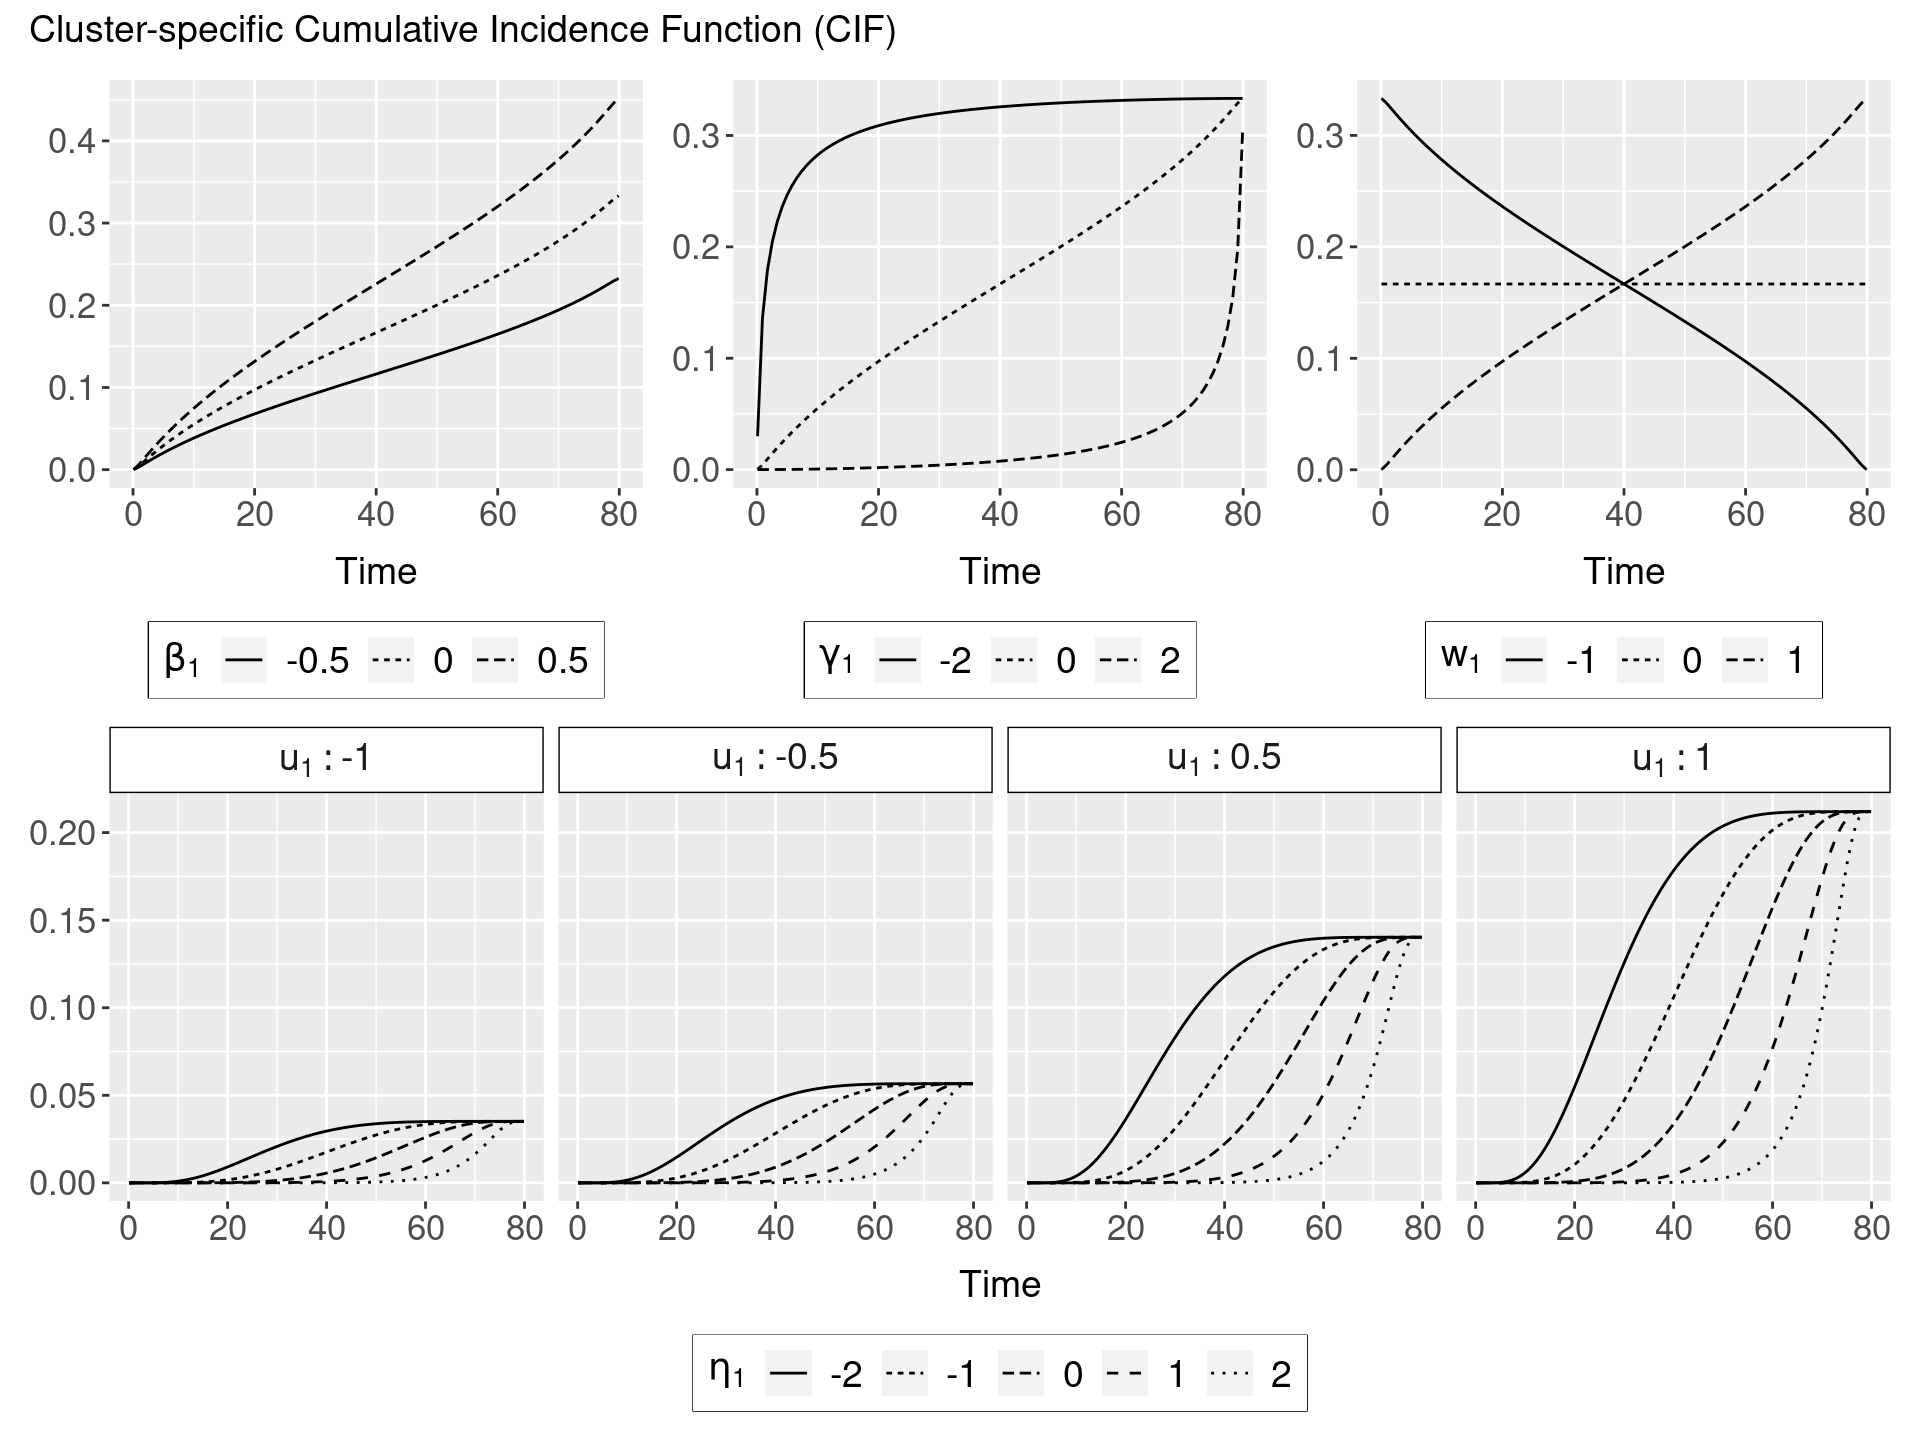
\includegraphics[width=\linewidth]{pics/cifstudy-1.png}
 \vspace{-0.75cm}
 \caption{Curve behaviors for different parameter settings, showing then
   the corresponding parameter effects in a cluster-specific cumulative
   incidence function (CIF).}
 \label{fig:cifcoefs}
\end{figure}

Remains to talk about the within-cluster dependence induced by the
latent effects in \(\bm{u}\) and \(\bm{\eta}\). To help in the
discussion, the bottom-plots on \autoref{fig:cifcoefs} illustrates the
cluster-specific CIF for a given failure cause in a model without
covariates, let us call it failure cause 1 (in total we have two). The
latent effects \(u_{1}\) and \(u_{2}\) always appear together in the
cluster-specific risk level, as consequency they have a joint effect on
the cumulative incidence of both causes. As we can see in
\autoref{fig:cifcoefs}, an increase in \(u_{k}\) will increase the risk
of failure from cause \(k\). The interpretation of
\(\text{cov}(\eta_{1},~\eta_{2})\) and \(\text{cov}(u_{1},~u_{2})\) is
straightforward, and those values are in most of the cases positive, as
said in \cite{SCHEIKE}. With regard to \(\text{cov}(u_{k},~\eta_{k})\),
negative values are the common situation. A negative correlation between
\(\eta_{k}\) and \(u_{k}\) imply that when \(\eta_{k}\) decreases,
\(u_{k}\) increases and conversely when \(\eta_{K}\) increases,
\(u_{k}\) decreases. In other words, an increased risk level is reached
quickly and a decreased risk level is reached later, respectively. With
regard to cross-cause correlation between \(\eta\) and \(u\), positive
values are the common situation where late onset of one failure cause is
associated with a high absolute risk of another failure cause.

\subsection{Model specification}
\label{multiGLMM}

The generalized linear mixed model (GLMM) for clustered competing risks
data is specified in the following hierarchical fashion. By simplicity,
we focus on two competing causes of failure but an extension is
straightforward. For two competing causes of failure, a subject \(i\),
in the cluster/family \(j\) and time \(t\), we have
\begin{align}
 y_{i j t} \mid \{u_{1j},~u_{2j},~\eta_{1j},~\eta_{2j}\}
 &\sim\text{Multinomial}(p_{1ijt},~p_{2ijt},~p_{3ijt})\nonumber\\
 \nonumber\\
 \begin{bmatrix} u_{1}\\u_{2}\\\eta_{1}\\\eta_{2} \end{bmatrix}
 &\sim\text{MN}
  \left(
   \begin{bmatrix} 0\\0\\0\\0 \end{bmatrix},
   \begin{bmatrix}
    \sigma_{u_{1}}^{2}&
    \text{cov}(u_{1},~u_{2})&
    \text{cov}(u_{1},~\eta_{1})&\text{cov}(u_{1},~\eta_{2})\\
    &\sigma_{u_{2}}^{2}&
    \text{cov}(u_{2},~\eta_{1})&\text{cov}(u_{2},~\eta_{2})\\
    &&\sigma_{\eta_{1}}^{2}&\text{cov}(\eta_{1},~\eta_{2})\\
    &&&\sigma_{\eta_{2}}^{2}
   \end{bmatrix}
  \right)\nonumber\\
 \nonumber\\
 p_{kijt}
 &=\frac{\partial}{\partial t}
  F_{k} (t \mid \bm{x},~u_{1},~u_{2},~\eta_{k})\label{eq:model}\\
 &= \frac{\exp\{\bm{x}_{kij}\bm{\beta}_{k} + u_{kj}\}}{
    1 + \sum_{m=1}^{K-1}\exp\{\bm{x}_{mij}\bm{\beta}_{m} + u_{mj}\}}
  \nonumber\\
 &\times w_{k}\frac{\delta}{2\delta t - 2t^{2}}~
  \phi\left(
   w_{k}
   \text{arctanh}\left(\frac{t-\delta/2}{\delta/2}\right)
   - \bm{x}_{kij}\bm{\gamma}_{k} - \eta_{kj}
  \right),\nonumber\\k = 1,~2.\nonumber
\end{align}
The probabilities are given by the derivative w.r.t. time \(t\) of the
cluster-specific CIF. The choice of a multinomial logistic regression
model ensures that the sum of all predicted cause-specific CIFs does not
exceed 1. Considering two competing causes of failure, we have a
multinomial with three classes. The third class exists to handle the
censorship and its probability is given by the complementary to reach
1. To better describe these curve behaviors we have
\autoref{fig:modelsample}.

\begin{figure}[H]
 \centering 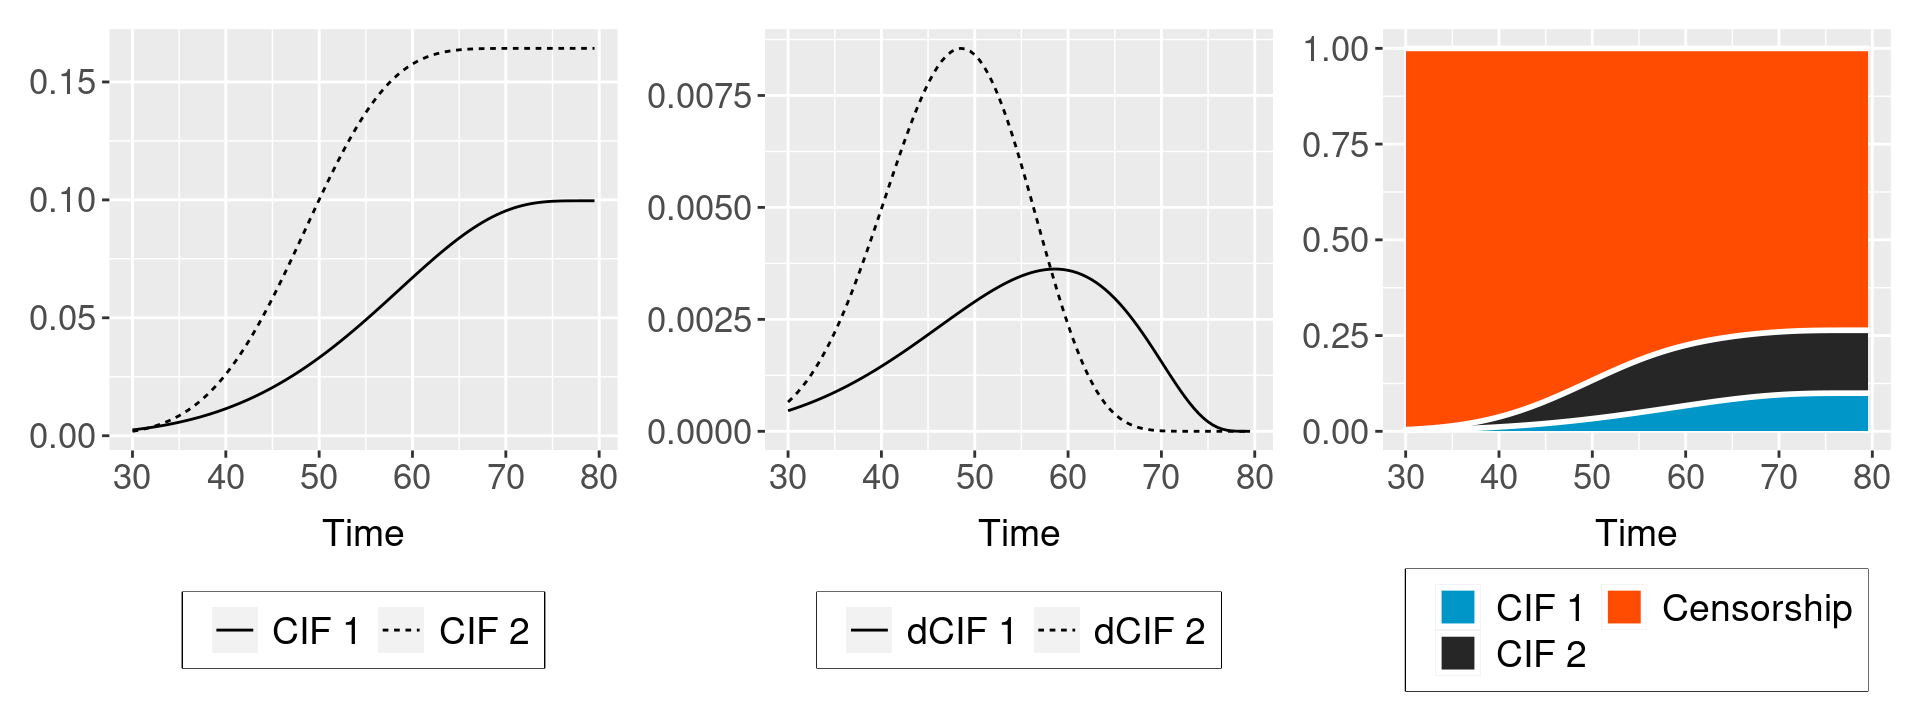
\includegraphics[width=\linewidth]{pics/modelsample-1.png}
 \vspace{-0.75cm}
 \caption{Cluster-specific cumulative incidence function (CIF) curves
   and their derivatives (dCIF) for a random scenario with two competing
   causes.}
 \label{fig:modelsample}
\end{figure}

This framework in \autoref{eq:model} results in what we call multiGLMM,
a multinomial GLMM to handle the CIF of clustered competing risks
data. For a random sample, the corresponding marginal likelihood
function in given by
\begin{align}
 L(\bm{\theta}~;~y)
 &= \prod_{j=1}^{J}~\int_{\Re^{4}}
    \pi(y_{j} \mid \bm{r}_{j})\times\pi(\bm{r}_{j})~\text{d}\bm{r}_{j}
    \nonumber\\
 &= \prod_{j=1}^{J}~\int_{\Re^{4}}
    \Bigg\{
    \underbrace{\prod_{i=1}^{n_{j}}~\prod_{t=1}^{n_{ij}}
    \Bigg(
    \frac{(\sum_{k=1}^{K}y_{kijt})!}{y_{1ijt}!~y_{2ijt}!~y_{3ijt}!}~
    \prod_{k=1}^{K} p_{kijt}^{y_{kijt}}
    \Bigg)}_{\substack{\text{fixed effect component}}}
  \Bigg\}\times\nonumber\\
 &\hspace{2cm}\underbrace{
   (2\pi)^{-2} |\Sigma|^{-1/2} \exp
   \left\{-\frac{1}{2}\bm{r}_{j}^{\top} \Sigma^{-1} \bm{r}_{j}\right\}
   }_{\substack{\text{latent effect component}}}
   \text{d}\bm{r}_{j}\nonumber\\
 &= \prod_{j=1}^{J}~\int_{\Re^{4}}
    \Bigg\{
    \underbrace{\prod_{i=1}^{n_{j}}~\prod_{t=1}^{n_{ij}}
    \prod_{k=1}^{K} p_{kijt}^{y_{kijt}}
    }_{\substack{\text{fixed effect}}}
   \Bigg\}\underbrace{
   (2\pi)^{-2} |\Sigma|^{-1/2} \exp
   \left\{-\frac{1}{2}\bm{r}_{j}^{\top} \Sigma^{-1} \bm{r}_{j}\right\}
   }_{\substack{\text{latent effect component}}}
   \text{d}\bm{r}_{j}\label{eq:loglik},
\end{align}
where \(\bm{\theta} = [\bm{\beta}~\bm{\gamma}~\bm{w}~\bm{\sigma^{2}}~
  \bm{\rho}]^{\top}\) is the parameters vector to be maximized. In our
framework, a subject can fail from just one competing cause or get
censor, at a given time. Thus, the fraction of factorials in the fixed
effect component is made only by 0's and 1's. The matrix \(\Sigma\) is
the variance-covariance matrix, which parameters are given by
\(\bm{\sigma}^{2}\) and \(\bm{\rho}\).

To each cluster \(j\) we have a product of two components. The fixed
effect component, given by a multinomial distribution with its
probabilities specified through the cluster-specific CIF
(\autoref{eq:cif}) and, the latent effect component, given by a
multivariate Gaussian distribution. To each subject \(i\) that composes
a cluster \(j\) we have its specific fixed effects contribution. The
likelihood in \autoref{eq:loglik} is the most general as possible,
allowing for repeated measures to each subject. Since all subjects of a
given cluster shares the same latent effect, we have just one latent
effect contribution multiplying the product of fixed effect
contributions. As we do not observe the latent effect variables,
\(\bm{r}_{j}\), we integrate out in it. With two competing causes of
failure we have four latent effects, a multivariate Gaussian
distribution in four dimensions. Consequently, for each cluster, we
approximate an integral in four dimensions. The product of these
approximated integrals results in the called marginal likelihood, to be
maximized in \(\bm{\theta}\).

\section{Estimation and inference}
\label{inference}

Our goal is to estimate the parameter vector \(\bm{\theta} =
[\bm{\beta}~\bm{\gamma}~\bm{w}~\bm{\sigma^{2}}~ \bm{\rho}]^{\top}\). The
likelihood for \(\bm{\theta}\) can be written as
\begin{equation}
 L(\bm{\theta} \mid \bm{y,u}) =
 \prod_{i=1}^{I}~\prod_{j=1}^{n_{i}}~
 f(y_{ij} \mid \bm{u}_{i}, \bm{\beta,\Sigma})~
 f(\bm{u}_{i} \mid \bm{\Sigma}).
 \label{eq:joint}
\end{equation}
From standard probability theory is easy to see that in the right-hand
side (r.h.s.) we have a joint density, consequently, \autoref{eq:joint}
represents what is called a full or joint likelihood function. The
latent effect \(\bm{u}\) is \textit{latent}, i.e. we do not observe
it. To handle this we use the Laplace approximation.

If we have a joint density we can just integrate out the undesired
variable resulting in
\begin{equation}
 \begin{aligned}
  L(\bm{\theta} \mid \bm{y}) &=
  \prod_{i=1}^{I}~\int_{\mathcal{R}^{\bm{u}_{i}}}
  \left[~\prod_{j=1}^{n_{i}}~
         f(y_{ij} \mid \bm{u}_{i}, \bm{\beta,\Sigma})~
         f(\bm{u}_{i} \mid \bm{\Sigma})
  \right]\text{d} \bm{u}_{i}\\
  &= \prod_{i=1}^{I}~\int_{\mathcal{R}^{\bm{u}_{i}}}~
  f(\bm{y}_{i}, \bm{u}_{i} \mid \bm{\theta})~\text{d} \bm{u}_{i},
  \label{eq:generalmarginal}
 \end{aligned}
\end{equation}
a marginal density that keeps the parameters \(\{\bm{\sigma^{2}}~
\bm{\rho}\}\) of the integrated variable. To handle this integration
step a clever choice is to take advantage of the exponential family
structure together with the Gaussian latent effects distribution. These
ideas converge to an adaptive Gaussian quadrature with one integration
point, also known as \textit{Laplace approximation}
\citep{molenberghs&verbeke,LA4H,tierney,corestats}.

We may approximate a analytically intractable integral in a way to
obtain a tractable closed-form expression allowing the numerical
maximization of the resulting marginal likelihood function
\citep{patrao}. The Laplace approximation has been designed to
approximate integrals in the form
\begin{equation}
 \int_{\mathcal{R}^{\bm{u}_{i}}}
 \exp\{Q(\bm{u}_{i})\} \text{d} \bm{u}_{i}\approx
 (2\pi)^{n_{\bm{u}}/2}~
 |{Q}''(\bm{\hat{u}}_{i})|^{-1/2}~\exp\{Q(\bm{\hat{u}}_{i})\},
 \label{eq:laplace}
\end{equation}
where \(Q(\bm{u}_{i})\) is a known unimodal bounded function, and
\(\bm{\hat{u}}_{i}\) is the value for which \(Q(\bm{u}_{i})\) is
maximized. A advantage of the Laplace approximation approach in a GLMM
is the exponential family structure. In a usual GLMM the response
follows a one-parameter exponential family distribution that can be
written as
\[
 f(\bm{y}_{i} \mid \bm{u}_{i}, \bm{\theta}) =
 \exp \left\{
  \bm{y}_{i}^{\top} (\bm{x}_{i}\bm{\beta} + \bm{z}_{i}\bm{u}_{i}) -
  \bm{1}_{i}^{\top}b(\bm{x}_{i}\bm{\beta} + \bm{z}_{i}\bm{u}_{i}) +
  \bm{1}_{i}^{\top} c(\bm{y}_{i})
      \right\},
\]
where \(b(\cdot)\) and \(c(\cdot)\) are known functions. This general
and easy to compute expression together with a (multivariate) Gaussian
distribution, highlights the convenience of the Laplace method. The
\(Q(\bm{u}_{i})\) function to be maximized can be expressed as
\begin{equation}
 \begin{aligned}
  Q(\bm{u}_{i}) &=
  \bm{y}_{i}^{\top} (\bm{x}_{i}\bm{\beta} + \bm{z}_{i}\bm{u}_{i}) -
  \bm{1}_{i}^{\top}b(\bm{x}_{i}\bm{\beta} + \bm{z}_{i}\bm{u}_{i}) +
  \bm{1}_{i}^{\top} c(\bm{y}_{i})\\
  &- \frac{n_{\bm{u}}}{2} \log (2\pi) -
     \frac{1}{2} \log |\bm{\Sigma}| -
     \frac{1}{2} \bm{u}_{i}^{\top}\bm{\Sigma}^{-1}~\bm{u}_{i}.
 \end{aligned}
\end{equation}
The approximation in~\autoref{eq:laplace} requires the maximum
\(\bm{\hat{u}}_{i}\) of the function \(Q(\bm{u}_{i})\). As we assume a
Gaussian distribution with a known mean for the latent effects, we have
the perfect initial guess for a Hessian-based maximization method, as
the Newton-Raphson (NR) algorithm. \cite{patrao} presents the generic
expressions for the derivatives required by the NR method, given by the
following:
\begin{equation}
 \begin{aligned}
  {Q}'(\bm{u}_{i}^{(k)}) &=
  \{\bm{y}_{i} - {b}'(\bm{x}_{i}\bm{\beta} + \bm{z}_{i}\bm{u}_{i}^{(k)})
  \}^{\top} - {\bm{u}_{i}^{(k)}}^{\top} \bm{\Sigma}^{-1},\\
  {Q}''(\bm{u}_{i}^{(k)}) &=
  - \text{diag}\{{b}''(\bm{x}_{i}\bm{\beta}
  + \bm{z}_{i}\bm{u}_{i}^{(k)})\} - \bm{\Sigma}^{-1}.
 \end{aligned}
 \nonumber
\end{equation}

The marginal log-likelihood function returned by the Laplace
approximation, to each individual or unit under study \(i\), is as
follows:
\begin{equation}
 \begin{aligned}
  l(\bm{\theta} \mid \bm{y}_{i}) =
  \log L(\bm{\theta} \mid \bm{y}_{i}) &= \frac{n}{2} \log (2\pi) -
  \frac{1}{2} \log
  \left| \text{diag}\{{b}''(\bm{x}_{i}\bm{\beta} +
                      \bm{z}_{i}\bm{\hat{u}}_{i})
                    \} + \bm{\Sigma}^{-1}
  \right|\\
  &+ \bm{y}_{i}^{\top}
     (\bm{x}_{i}\bm{\beta} + \bm{z}_{i}\bm{\hat{u}}_{i}) -
     \bm{1}_{i}^{\top}
     b(\bm{x}_{i}\bm{\beta} + \bm{z}_{i}\bm{\hat{u}}_{i}) +
     \bm{1}_{i}^{\top} c(\bm{y}_{i})\\
  &- \frac{n_{\bm{u}}}{2} \log (2\pi) -
     \frac{1}{2} \log |\bm{\Sigma}| - \frac{1}{2}
     \bm{\hat{u}}_{i}^{\top}\bm{\Sigma}^{-1}~\bm{\hat{u}}_{i},
 \end{aligned}
 \nonumber
\end{equation}
that can now be numerically maximized over the model parameters
\(\bm{\theta} = [\bm{\beta}~\bm{\gamma}~\bm{w}~\bm{\sigma^{2}}~
  \bm{\rho}]^{\top}\) using a quasi-Newton method as the
Broyden-Fletcher-Goldfarb-Shanno (BFGS) algorithm \citep{nocedal&wright}
or the PORT routines \citep{PORTpaper,PORTreport}, all available in the
R \citep{R21} statistical software.

We use an efficient Laplace approximation routine implemented in
\texttt{TMB} \citep{TMB}. Besides state-of-art linear algebra libraries
and the possibility of performing the computations in parallel,
\texttt{TMB} also offers an efficient implementation of automatic
differentiation \citep{nocedal&wright,corestats,peyre}, the state-of-art
in gradients computation. In \texttt{TMB} the user should write its
likelihood function in a \texttt{C++} template file and then load it on
R. This last characteristic makes \texttt{TMB} general (a vast range of
models being allowed to be written) and powerful (low-level \texttt{C++}
model implementation).

\section{Simulation studies}
\label{simulation}

To verify the practical viability of our model we performed an extensive
simulation study. As main complicator factors, we may mention the
competing causes un balancement, where we typically have much more
censorships than actual failures; and the high dimensionality problem,
having a considerable number of parameters to estimate in both fixed and
latent effects layers.

One of the main questions surrounding our model that we tried to tack
down in this study was, if even when in the possession of a high
correlated sample in the latent field, we are able to estimate all
variance and covariance parameters.

One of the main questions surrounding our model that we tried to tack
down in this study was, if even when in the possession of a high
correlated sample in the latent field, we are able to estimate all
variance and covariance parameters. To answer this question we worked
with four different models, with each one differentiating from the other
in terms of latent effects structure. We had a model with (i) latent
effects only on the risk level; (ii) only on the failure time trajectory
level; (iii) on both levels but without cross-correlations, called a
blog-diag model; and (iv) a model with all possible correlations
presented, called as a complete model. A visual representation of these
latent effects structures is presented in \autoref{fig:matrix} in terms
of the corresponding variance-covariance matrices.

\begin{figure}[H]
 \centering 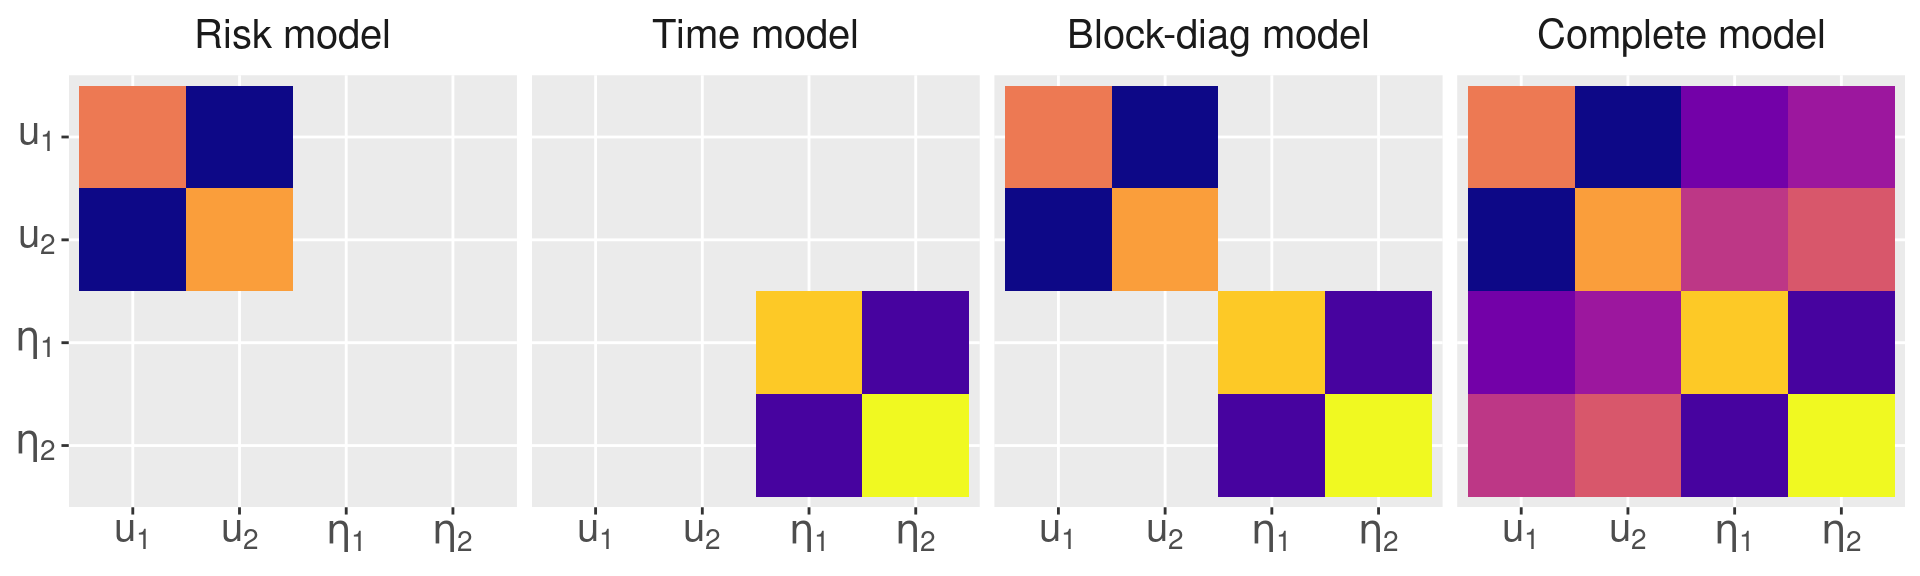
\includegraphics[width=\linewidth]{pics/matrix-1.png}
 \vspace{-0.75cm}
 \caption{Simulation study variance-covariance matrix model designs,
   considering two competing causes of failure and consequently, four
   latent effects.}
 \label{fig:matrix}
\end{figure}

\section{Discussion}
\label{discussion}

\section*{Supplementary material}

\bibliographystyle{dcu}
\bibliography{references}

\end{document}
